%0       1         2         3         4         5         6         7         8
%2345678901234567890123456789012345678901234567890123456789012345678901234567890

%=======================================================================
% \documentclass[12pt]{article}
\documentclass[10pt]{article}
%=======================================================================

% INCLUDE DEVELOPMENT TEXT

\newcommand{\devel}[1]{\textbf{#1}}

% EXCLUDE DEVELOPMENT TEXT

% \newcommand{\devel}[1]{}


%=======================================================================
% Document layout
%=======================================================================

\setlength{\topmargin}{0.0in}
\setlength{\oddsidemargin}{0.0in}
\setlength{\evensidemargin}{0.0in}
\setlength{\textwidth}{6.0in}
\setlength{\textheight}{9.0in}

%=======================================================================
% Packages
%=======================================================================

\usepackage{wasysym}
\usepackage{epsfig}
\usepackage{url}

%=======================================================================
% Commands
%=======================================================================

\newcommand{\cello}{\textsf{Cello}}
\newcommand{\enzo}{\textsf{Enzo}}
\newcommand{\lcaperf}{\textsf{lcaperf}}
\newcommand{\lcatest}{\textsf{lcatest}}

\newcommand{\code}[1]{\textsf{#1}}

\newcommand{\note}[1]{\devel{\eighthnote\ \textit{#1} \\}}
\newcommand{\pargraph}[1]{\devel{\P\ \textbf{#1} \\}}

\newcommand{\todo}{\devel{$\circ$}}
\newcommand{\done}{\devel{$\bullet$}}
\newcommand{\halfdone}{\devel{\textcolor{gray}{$\bullet$}}}

\newcommand{\PROJECT}{\cello}

\newcommand{\TITLE}[3]{
\title{ {\huge \PROJECT\ #1}  \\ \vspace{0.1in}
     {\small Document Version: \textbf{#3}} \vspace{-0.1in}
    }
\author{      #2 \\
        Laboratory for Computational Astrophysics\\
        University of California, San Diego}
\maketitle}

%=======================================================================


% Project summary
% Introduction
%    Extreme parallelism
%    Extreme AMR
%    Existing AMR frameworks
%       PARAMESH
%       Chombo
%       SAMRAI
%       GADGET
% Software requirements
% Software design
%    High level components
%    Data structures
%       Patch coalescing  for ``shallow'' AMR
%       Targeted refinement with backfill for ``deep'' AMR
%    Task scheduling
%    Load balancing
% Implementation
%    Parallelism
%    Fault tolerance
%    Software implementation
% Development plan
% Milestones and deliverables

\usepackage{natbib}

%=======================================================================

\begin{document}

\tableofcontents
%\Large
\renewcommand{\pargraph}[1]{}

\nocite{StSh09} % Scalability challenges for massively parallel {AMR} applications
\nocite{WiHy03} % Enhancing scalability of parallel structured {AMR} calculations
\nocite{GuWi06} % Parallel clustering algorithms for structured {AMR}
\nocite{BuGh08} % Towards adaptive mesh {PDE} simulations on petascale computers
\nocite{BaBu09} % MPI on a million processors

\nocite{LaTa06} % hierarchical load balancing

%=======================================================================
\TITLE{A Software Framework for Extreme Adaptive Mesh Refinement}{James Bordner}{$Rev$}
%=======================================================================

%
%
%

% Keywords
%
%    AMR
%    applied mathematics
%    collaborative software environments
%    computer science technologies
%    exascale
%    extreme scale
%    failure avoidance
%    failure effects avoidance
%    fault tolerance
%    GPU
%    hierarchical
%    HPC
%    memory hierarchy
%    multicore
%    multiphysics
%    multiscale
%    one-sided communication
%    performance tuning
%    petascale
%    PGAS
%    research goals
%    resilient software
%    UPC
%    virtual processes
%
% suggestions
%
%    preliminary results
%    good references critical; only give great references
%    use rfp keywoards
%    sustainability--what happens when money ends
%    sales document not technical manual
%    visit agency web site for similar funding
%    make benefits clear
%    write for evaluators
%    justify and support all claims
%    active voice: strong subjects and active verbs
%    first paragraph sentence conveys topic
%    65 characters per line
%    duplicate information instead of cross reference
%    use graphics and tables
%    short text with bullets
%    stay on topic
%
% more suggestions
%
% [ compelling, organization goals and success, relevence to agency]
% problem statement--needs assessment
%     motivation / history
%       enzo
%       cello project
%       decoupled framework
%       well-aware of scalability issues
%       understand importance of performance / scalability of all components
%     purpose
%     beneficiaries
%     what is being done
%     what we will do
% objectives: table with direct items
% development plan
%    chart with timelines
%    decision points
%    milestones
%    tasks
% methods and design
%     use flow charts and diagrams to break up text
%     justify course of action
%     highlight innovative features
% past experience
% management approach
%   quality control
%   emphasize performance management
%   technological systems in place


%=======================================================================
\section{Project Summary}  \label{s:summary}
%=======================================================================


\pargraph{Proposal} 
%
We propose to develop a new parallel software framework for adaptive
mesh refinement (AMR).  
%
A distinguishing characteristic relative to existing AMR libraries and
frameworks is the aggressive pursuit of extreme scalability in terms
of software data structures and hardware parallelism from the
beginning.
%
The design will be forward-looking, targeted not just at the largest
existing supercomputers, but also future HPC platforms as they evolve
through the petascale era and into the exascale.
%
The proposed AMR framework will enable application developers to
write multiphysics applications for simulating phenomena on an
unprecidented range of spacial and temporal scales.

\pargraph{multiple parallel technologies}
%
Parallelization will be primarily data parallel, with task
parallelization also available to augment the data parallelism.
%
A wide variety of parallelization technologies will be supported from
the start, including both one- and two-sided message passing via the
MPI~\cite{wwwmpi} library, the partitioned global address space (PGAS)
approach via the UPC~\cite{@@@UPC} language, shared memory parallel
programming using OpenMP compiler directives, and the message-driven
processor virtualization approach provided by the \charm\
framework~\cite{@@@Charm}.
%
Hierarchical parallelism will be supported though select hybrid
approaches, such as MPI with OpenMP, and MPI with UPC.

\pargraph{Load balancing}
%
Dynamic load balancing of parallel tasks will be hierarchical, which
will improve mapping of the software data structures to the
hierarchical components of the target computational platforms (i.e.
compute nodes, sockets, cores).~\cite{@@@LAN-DLB}.

\pargraph{AMR fields + particles}
%
The AMR data structures will be implemented using a fully distributed
generalization of the octree data structure.  Tree nodes will be
associated with both logically Cartesian grids and particles, so both
Eularian and Lagrangian (and hybrid) methods can be implemented.

\pargraph{extreme scalability through localization}
%
Extreme parallel scalability will be pursued by localizing the
individual AMR patch / block tasks as much as feasible by aggressively
removing all unnecessary global data, global communication, and global
coordinate systems.  For the latter, since fixed-size integers and
floating-point values limit particle global position accuracy and
global index ranges, localizing the problem will also improve scaling
of the data structures without having to resort to 64-bit or higher
scalars.

\pargraph{fault tolerance} Fault tolerance and software
resilience are also crucial factors at extreme scales.  The checkpoint
/ restart to disk paradigm is known to be ultimately unscalable, so we
will support other alternatives, including checkpoint to memory.  Our
framework will be designed to be resistent to memory, compute
component, network, disk, and software failures.

\pargraph{deliverables} 
%
We plan to make this framework freely available for use by the
research community.  The result of this project will be software
framework capable of allowing application developers write extremely
scalable multi-resolution multi-physics applications.

\begin{verbatim}
\cite{StSh09} quote
load balancing and communication are often cited as the main
barriers to AMR scaling, but instead ``...many of the scaling problems related to early design decisions''
\end{verbatim}
%=======================================================================
\section{Introduction} \label{s:intro}
%=======================================================================


The \cello\ Project began as an effort to redesign the parallel data
structures of the astrophysics and cosmology application \enzo\
\cite{OsBr04}.  \enzo\ was conceived in the early 1990's by Michael
L.~Norman and Greg Bryan, and implemented using structured
(patch-based) adaptive mesh refinement (SAMR) \cite{BeCo89}.  It
incorporated a modified high-order Piecewise Parabolic Method (PPM)
solver \cite{WoCo84b} for hydrodynamics, and a Particle-Mesh (PM)
method \cite{@@@PM} for dark matter dynamics.  So far in its 15 year
lifetime, \enzo\ simulations have led to important scientific
contributions to the fields of astrophysics, cosmology, and
turbulence.

\enzo\ scales well up to $\approx 10^4$ to $\approx 10^5$ processes,
depending on the problem.  Efforts to improve its scalability beyond
this have become increasingly difficult, due to the increasing
invasiveness of the desired changes and the increasing complexity of
the code base.  The \cello\ Project aims to improve on \enzo\ in three
ways: improved software development process, object-oriented design
and implementation, and overhauled distributed AMR infrastructure.
The physics capabilites, which are continually being improved and
refined in \enzo, will be retained in \enzo II.

\begin{verbatim}
Motivation
Forward-looking
Supercomputer trends
Innovative / core ideas
  hierarchical load balancing
  separate scheduling of communication and computation
  flexible dynamic data organization for comm, comp, disk
  task size / count control
  gang scheduling for GPU support
  task parallelism: pipeline computational methods to increase parallelism
  AMR: patch coalescing
  AMR: targeted refinement by 4, 8 with backfill
  aggresive localization
    only store local coordinates for particles
    only store local patch connectivity
  fault tolerance @@@
  multiple parallelization technologies with flexible hybrid support
     why?  
        experimentally 
        forces encapsulation of parallelism; 
        likely improves ease of adapting future parallel strategies
  designing with extreme scale in mind from the beginning
\end{verbatim}

\begin{verbatim}
upcoming systems
   BW
   ...
   ...
   core counts
   extrapolate top500 10 years
   what this means for extreme scalable AMR + particles
\end{verbatim}

\begin{verbatim}
refined  / borrowed ideas
  fully distributed AMR datastructure
  patch block registers for improved computing / user interface flexibility
  communication flux registers (\chombo) for communication
  guard cells allocated when needed
  localized fully-adaptive time steps (no global reductions) (refined)
\end{verbatim}


\note{Extreme parallelism}

\begin{verbatim}
distributed data placement
   hierarchical
   different needs for different tasks
      compute
      store
\end{verbatim}

\begin{verbatim}
parallel computation
   data parallelism (SPMD)
   task parallelism
   cooperative parallism (MPMD)
\end{verbatim}

\begin{verbatim}
parallel technology
   MPI / charm++  / UPC / OpenMP / GPU
\end{verbatim}

\begin{verbatim}
heterogeneous hardware computation
   GPUs, cores
\end{verbatim}

\begin{verbatim}
load balancing
   keep all cores busy
   between shared memory compute nodes -- memory
   within shared memory compute nodes -- computation
\end{verbatim}

\begin{verbatim}
task definition
   size
   count
   hierarchical
\end{verbatim}

\begin{verbatim}
task scheduling
   hierarchical / multiscale
     distributed versus shared memory
   communication / computation
   decouple data distribution from task scheduling
\end{verbatim}

\begin{verbatim}
reducing synchronization / increasing task independence
\end{verbatim}

\begin{verbatim}
software resiliency / fault tolerance
\end{verbatim}

\begin{verbatim}
checkpointing / restart
   trend: disk progressively slower
\end{verbatim}


\pargraph{load balancing summary}
We will use a hierarchical dynamic load balancing approach, with
support for balancing with respect to multiple metrics (memory use,
computational load, etc.) for different hierarchical computational
components (compute node, socket, etc.), with different rebalancing
frequencies for different levels.

\note{Extreme AMR}

\begin{verbatim}
parallel scalability issues
   global synchronization / reductions
   load balancing
   I/O
   fault tolerance
   ``OS jitter'' and memory management can lead to load imbalances
        independent of application\cite{StSh09}
\end{verbatim}

\begin{verbatim}
AMR-specific parallel scalability issues
   elliptic
   remeshing--especially SAMR
   load balancing
   time step determination
\end{verbatim}

\begin{verbatim}
AMR datastructure scalability
   breadth--number of grid patches
   depth--range of multi-resolution
   floating point precision issues
   floating point range issues
   integer range issues
\end{verbatim}

%-----------------------------------------------------------------------
\subsection{Existing AMR frameworks} \label{ss:review}
%-----------------------------------------------------------------------

\begin{verbatim}
 http://people.sc.fsu.edu/~tomek/AMR/index.html
 *   Adaptive Mesh Refinement Software for Hyperbolic Conservation Laws, Marsha Berger
 * Adaptive Mesh Refinement and Parallel Computing, John A. Trangenstein, Mathematics Department, Duke University.
 * Amrita, James Quirk.
 * AMR1D, a simple adaptive mesh refinement code for solving the one-dimensional Euler equations on an unstructured grid.
 * AMRCART, The AMRCART MHD Code, Rolf Walder.
 * AMRCLAW, Adaptive Mesh Refinement + CLAWPACK. AMRCLAW is a joint project between Randy LeVeque and Marsha Berger.
 * AMRMHD3D, 3-D AMR code with FCT MHD solver.
 * AMROC, Blockstructured Adaptive Mesh Refinement in object-oriented C++, Ralf Deiterding.
 * AMRPoisson, Solving Poisson's Equation using Adaptive Mesh Refinement (AMR), Computational Fluid Dynamics, Dept. of Mechanical Engineering, U.C. Berkeley.
 * ARMS, 3-D AMR code with FCT MHD solver.
 * BEARCLAW, general purpose software package for solving time-dependent partial differential equations, Sorin Mitran, Applied Mathematics Program, The University of North Carolina at Chapel Hill.
 * BSAMR, Block Structured Adaptive Mesh Refinement, Daniel D. Wake, College of Engineering, UC Davis.
 * Cactus, The Cactus Code Server, Max Planck Institute for Gravitational Physics (Albert Einstein Institute), Max Planck Society.
 * Cart3D, Michael J. Aftosmis, Numerical Aerospace Simulation (NAS) Division Systems, NASA Ames Research Center
 * CTH, 3-D multi-material Eulerian AMR code from Sandia (export controlled).
 * Enzo, Cosmological Simulation Code, Laboratory for Computational Astrophysics, UCSD.
 * FEMLAB, FEM with automatic error control for two-dimensional convection-diffusion-absorption problems.
 * FLASH, multi-physics 3-D octree AMR parallel code.
 * Gerris Flow Solver, incompressible fluid flow with arbitrarily complex solid boundaries and adaptive mesh refinement, Stephane Popinet.
 * GrACE, Grid Adaptive Computational Engine, Manish Parashar.
 * NIRVANA, 3-D MHD AMR code, Udo Ziegler.
 * \paramesh, 3-D octree AMR parallel code.
 * RACOON, Institute for Theoretical Physics I, University of Bochum.
 * SARA, A Solution Adaptive Remeshing Algorithm for structured grids, Dave Banks, Center for CFD, Dept. of Mech & Aero Eng, UC Davis.
 * Solution-Adaptive Grids, W. M. Keck Foundation CFD laboratory, University of Michigan.
 * SUUMA3D, Scalable Unstructured Mesh Algorithms and Applications, MCS ANL. 
\end{verbatim}

There are numerous AMR frameworks, libraries, and applications, each
with different design goals and decisions, data structures, AMR
algorithms, parallelization strategies, and parallel performance and
scaling.  Perhaps the top three most successful and closely related to
our proposed effort are \paramesh\ (\cite{MaOl00} \nocite{OlMa05}
\nocite{Ol06}), \chombo\  (\cite{wwwchombo} \cite{CoGr09}), and \samrai
(\cite{@@@}).  Other notable software include Clawpack (@@@), GrACe / DAGH
(@@@), ALPS (\cite{BuBu09}), and Carpet (@@@).

limitations of existing AMR libraries / frameworks

GADGET-2: Preeminent cosmological TreeSPH simulation code
DAGH (1998)

\begin{verbatim}
SCALING

\samrai\ scalability of parallel clustering algorithm up to 16384~\cite{GuWi06}
\chombo: demonstrated scalability up to 8192 processors~\cite{StSh09},
        and goals to continually improve scaling by a factor of 100 in 5 years~\cite{St09} (@@@public slides?).
  
FLASH: \paramesh\ re-gridding does not scale well
       I/O costly despite not being particularly inefficient
ALPS: scalable up to 32K cores and 4 billion ellements~\cite{BuGh07}
     (uses ``time windows''~\cite{SuWh04} to improve re-gridding performance,
      which requires ``...repeat[ing] the numerical integration of the PDEs over a time window one or more times to accumulate error estimates''. Depending
     on the PDE integration cost, this could improve apparent scalability
     by increasing task size )
\cite
\end{verbatim}

%-----------------------------------------------------------------------
\subsubsection{\paramesh} \label{sss:paramesh}
%-----------------------------------------------------------------------

\nocite{wwwparamesh}
\nocite{MaOl00} % PARAMESH requested references
\nocite{OlMa05}
\nocite{Ol06}

The \paramesh\ software was developed at the NASA Goddard Space Flight
Center and Drexel University.

It is an octree-based AMR framework

\paramesh\ grid blocks can be arbitrary constant even size $($\code{NXB},\code{NYB}, \code{NZB}$)$~\cite{wwwparamesh}.

Due to a loss of funding, \paramesh\ is not currently supported.

%-----------------------------------------------------------------------
\subsubsection{\chombo} \label{sss:chombo}
%-----------------------------------------------------------------------



\chombo~\nocite{CoGr09} is an MPI-parallel structured AMR (SAMR)
framework in active development by the Applied Numerical Algorithms
Group of Lawrence Berkeley National Lab.  It supports hyperbolic,
elliptic, and parabolic methods. Its high-level design consists of
five loosely-coupled components: \code{BoxTools} for set calculus on
point sets and unions of rectangles, \code{AMRTools} for interprocess
communication between AMR levels, \code{AMRTimeDependent} for
advancing the solution using adaptive time steps,
\code{AMRElliptic} for the multigrid-based solution of elliptic AMR
problems, and \code{EBTools} for embedded boundaries.  A sixth
component, \code{ParticleTools} for particle processing, is not
currently available due to re-engineering of the
component~\cite{wwwchombo}.

\chombo\ is parallelized using MPI.  An effort to modify \chombo\ to
use UPC was undertaken~\cite{We04}.
Distributed data in \code{LayoutData}, \code{BoxLayoutData}, and
\code{LevelData} containers.  \chombo\ provides a load balancing
algorithm, and also allows the user to provide their own.

\chombo\ is very scalabale, and designed to run both hyperbolic and
elliptic problems on 10,000 processors.

In \chombo, all processes store $O(N)$ data, including all patch
extents and process assignments.  Although the size has been
aggressively reduced to an impressive $\approx 50$ bytes per
patch~\cite{CoKe07}, this still represents an eventual scaling
impediment for \chombo.

Berger-Rigoutsos 


\pargraph{\chombo\  data distribution and load balancing}


%-----------------------------------------------------------------------
\subsubsection{\samrai} \label{sss:samrai}
%-----------------------------------------------------------------------

[2001]

good scaling for numerical and data communication
poorer scaling in adaptive meshing and communication schedule construction 

%-----------------------------------------------------------------------
\subsubsection{\gadget } \label{sss:gadget}
%-----------------------------------------------------------------------


\newpage
%=======================================================================
\section{Software Requirements} \label{s:requirements}
%=======================================================================


The software will be a framework that allows application developers to
write multiphysics PDE applications that span a wide range of
resolutions, and that require an amount of computational resources,
memory, and storage only available on the largest available HPC
platforms.  All software in the system will be released as open
source.  Below we describe a subset of the software requirements
specification, though more qualitatively than quantitatively.

Problems that the framework will support include systems of nonlinear
PDE's, including hyperbolic conservation laws and elliptic equations.
Specifically in terms of the astrophysics / cosmological application
\enzoii\ driving the development, the framework will support solving
Euler's equations of hydrodynamics, magnetohydrodynamics,
radiation-hydrodyanmics, and Poisson's equation for self-gravity.

Spacial dimensions will include $3$D, but the framework will also
support $1$D and $2$D, primarily for test problems.  Supported
algorithms (the implementations of which are not in the scope of the
framework, but are in the scope of the user functions and \enzoii\
driving application) include Eulerian mesh-based methods
(e.g.~PPM~\cite{WoCo84b}), Lagrangian particle-based methods, and
hybrid particle-mesh (e.g.~PPPM~\cite{HoEa88}) methods.

Optionally, we may also support multiple simulations run
simultaneously; this could allow for inter-simulation inline analysis
for parameter studies that would otherwise be infeasible due to
excessive data storage requirements.


%-----------------------------------------------------------------------
\subsection{Adaptive mesh refinement} \label{ss:require-amr}
%-----------------------------------------------------------------------

The AMR data structure must be highly scalable in both breadth and
depth, supporting at least @@@ $10^8$ grid patches and @@@ $60$ levels
of refinement.  The extreme number of possible grid patches indicates
that the data structure must be at least partially distributed.  The
extreme possible depth indicates that there must be no precision or
range issues with global floating point positions or global integer
indices.  The great range in resolutions also suggests that the
framework should support flexible numerical scaling at different mesh
levels, to reduce floating point errors and prevent underflow or
overflow errors.

The AMR data structure should also be ``efficient'' at adapting in
terms of the number of grid patches.  In particular, if much of the
region consists of large areas that require the finest grid level,
then the number of patches covering those regions should not be
excessive.  We note that this requirement essentially eliminates
fixed-size patches, which most octree-based AMR approaches use.  It
also indicates that when AMR is not used, the AMR data structure should
require nominal additional resources.

The AMR data structure should also be efficient and scalable in terms
of all of its operations, including coarsening, refining, and locating
neighboring patches.  Note that this indicates that some sort of
spacial data structure or other optimization, such as octrees,
chaining meshes, or caching intersection lists~\cite{StSh09}, will be
required.

The mesh hierarchy should dynamically adapt to problem features as
specified by the user.  Local changes in resolution should remain
bounded, e.g.~neighboring patches must be at most one level different,
to maintain numerical accuracy.  Also, refinement of symmetric
problems should retain logical symmetry (cells but not necessarily
patches) in the AMR data structure, to help prevent asymmetries in the
numerical solution.


%-----------------------------------------------------------------------
\subsection{Mesh data} \label{ss:require-fields}
%-----------------------------------------------------------------------

Multiresolution data fields defined on logically Cartesian meshes,
used for Eulerian mesh-based and hybrid particle-mesh methods, will be
supported by the AMR data structure.  The number and identification of
fields will be flexible and declared by the user: no assumptions will
be made on specific data field names or properties in the framework.

Stencil-based discretization methods will of course be supported,
which indicates that a layer of ``ghost'' or ``guard'' cells will be
required for computations.  The framework will allow flexible layers
of ghost zones, up to at least three zones deep.  Furthermore, the number and
depth of ghost zones may depend on the specific field, and ghost zones
may or may not be permanantly stored.

Data fields may be single or double precision, and different fields
may have different precisions, depending on the relative importance of
storage and accuracy for individual fields.  The framework will also
support scaling different fields by different amounts at different
levels, to improve the numerical behavior of user methods on an
extreme range of scales.

The framework will also allow for user methods to operate on
individual patches, all patches within a level, or all patches in the
hierarchy.  The motivation is that the most scalable and accurate
methods for coupled hyperbolic and elliptic problems defined on AMR
hierarchies typically involve solving linear systems defined both
within a single level and on the entire AMR hierarchy~\cite{MiCo07}.


%-----------------------------------------------------------------------
\subsection{Particle data} \label{ss:require-particles}
%-----------------------------------------------------------------------

In addition to mesh data, particle data will also be supported, for
use in Lagrangian particle-based and hybrid particle-mesh methods.
Multiple groups of particles will be supported, e.g.~\enzoii\ will
include ``star'' particles, dark matter particles for collisionless
gravitational dynamics, tracer particles for analysis and
visualization, etc.  All particles will have position, and different particle
groups will have different user-defined attributes associated with them, such
as velocity, mass or momentum, etc.

Extreme particle counts will be supported, indicating that particles
must be at least partially distributed.  Since many algorithms on
particles require particle proximities, operations such as finding
nearest neighbors must be efficient.  This indicates that an efficient
distributed spacial data structure must be used, such as an octree or
orthogonal recursive bisection.  Also, since hybrid particle-mesh
methods will be supported, locating all particles within a mesh, and
locating the mesh for a given particle, must be efficient.


%-----------------------------------------------------------------------
\subsection{User functions} \label{ss:require-user}
%-----------------------------------------------------------------------

While the framework supports adaptive mesh refinement for both mesh
and particle data, algorithms and other problem-dependent functions
must be provided by the user.  User functions may be either Fortran or
C (or C++).  

The main functions users supply will be numerical algorithms for
advancing a patch, hierarchy level, or full hierarchy one time step.
Inline-analysis and visualization functions may also be provided by
the user.  Patch-based user functions will have access to the
associated mesh and particle data, plus a bounding layer of ``ghost''
or ``guard'' zones on the mesh, as well as an analagous layer of
nearby particles.

Other user functions provided by the user will include functions for
imposing inter-level constraints such as flux correction, functions
for interpolating data to a finer mesh or for restricting data to a
coarser mesh, and functions for evaluating refinement criteria to
refine or coarsen a given patch.


%-----------------------------------------------------------------------
\subsection{Run-time parameters} \label{ss:require-parameters}
%-----------------------------------------------------------------------

Run-time parameters, such as those defining the domain, initial
conditions, AMR data structure properties, parallelism approach,
numerical method parameters, mesh fields and particle groups, etc.,
will be specified using a single or multiple included parameter files.
User code will have access to all parameters, including those
associated with the framework.

The parameter file grammar and data types should be powerful enough to
specify user problems; in particular, it should be powerful enough to
define any existing \enzo\ test problem for the \enzoii\ driving
application, despite not having problem-specific parameters and
initialization implemented in the code.  Since initial conditions are
typically specified by setting fields equal to different numerical
expresions in different subregions of the domain, the parameter file
grammar must be able to support both arbitrary scalar expressions for
field values, and arbitrary logical expressions involving spacial
variables (e.g.~\code{x}, \code{y}, and \code{z}) for specifying
subregions of the domain.  Common data types such as scalars, strings,
and lists or arrays should be supported as well.  Field and particle
initial conditions may also be defined in terms of user code or data
files.

The range of parameters should be both broad and deep, allowing
flexible definition of simulations and detailed control of data
structures and methods.  The expected large number of parameters
indicates a hierarchical organization of parameters, e.g.~explicit
grouping of parameters based on related functionality to improve
parameter file readability.

%-----------------------------------------------------------------------
\subsection{Parallelism} \label{ss:require-parallel}
%-----------------------------------------------------------------------

The framework will be highly scalable, so parallelism is a key
feature of the software.  There will be no fundamental limit on
process or thread counts (i.e.~no hard-coded \code{MAX\_PROCESSORS} constant).

Parallelism will include both distributed and shared memory models, as
well as hybrid parallelism.  This implies that many sections of both
the framework and user code must be thread safe.  The distributed
memory model is necessary for running efficiently on platforms that do
not support a single virtual memory address space, and the shared
memory model helps reduce memory consumption by allowing shared data
between threads instead of duplicating data between processes.

Parallel task definition is crucial to both performance and scaling of
parallel applications---there must be enough tasks to provide
sufficient parallelism, individual tasks must be large enough that
overhead does not dominate computation, and tasks must be defined such
that there is not excessive inter-task communication.  We note that
this requirement can conflict with standard AMR data structures if
individual AMR patches are taken to be individual parallel tasks.
This is because patch counts and sizes are dependent functions of
resolution requirements, which leaves parallelism to be only
indirectly controllable through AMR parameters, such as limits on the
range of allowable patch sizes.  This indicates that relaxing the
constraint of defining parallel tasks as individual AMR patches could
be beneficial.

The framework will directly support multiple levels of parallelism,
not just at the distributed memory / shared memory levels.
Specifically, the framework will support up to four levels of
parallelism, for example corresponding to hardware cabinents, nodes,
processors, and cores.  We expect that this will improve both
efficiency and scalability, by allowing more flexible mapping of the
distributed data structures onto the hierarchical parallel hardware,
and by reducing the size of groups of intercommunicating
procesess~\cite{BaBu09}.

%-----------------------------------------------------------------------
\subsection{Load balancing} \label{ss:require-balance}
%-----------------------------------------------------------------------

Dynamic load balancing / task migration is critical for parallel
performance of AMR, due to the dynamically changing workload
distributed across nodes with limited memory and potentially millions
of computational cores.  Dynamic load balancing must therefore be
efficient, reliable, and effective.  Since we will directly support
multiple levels of hardware parallelism, this indicates that a
hierarchical load balancing approach should be used,
e.g.~\cite{LaTa06}.  This would allow for balancing between different
parallel levels at different frequencies, and balancing with respect
to different metrics (e.g.~stress balanced computation between cores
and balanced memory usage between nodes).

%-----------------------------------------------------------------------
\subsection{Task scheduling}\label{ss:require-schedule}
%-----------------------------------------------------------------------

Task scheduling must also be efficient, minimizing overhead and
maximizing throughput.  Again, a hierarchical scheduling approach may
be used.  Since we want to at least indirectly support GPU programming
in user code, we will want to support scheduling large groups of
concurrent tasks to keep the GPU's busy.

  
%-----------------------------------------------------------------------
\subsection{Interfaces} \label{ss:require-interfaces}
%-----------------------------------------------------------------------

The framework must be able to communicate with users while running, to
provide clear output of the state and progress of the simulation.
This should include an estimate of progress, performance, list of any
warnings or errors, as well as method-specific information such as
solver iterations or method-specific warnings or errors.  This
indicates that user code as well as the \cello\ framework should have
access to functions for communicating values to users in a running
simulation.

The mode of output should not be limited to text, but should include
support for generating simple plots of data fields and particle
groups, and graphs indicating the progress or performance of the
simulation, and the historical output of important values indicating
correctness or progress, such as total mass, $||\nabla \cdot B||$, and
time step size.

All output should be easily viewable, at varying levels of detail from
high-level summary levels to more in-depth detailed levels.  This
could indicate the framework periodically writing a set of dynamically
changing web pages.


%-----------------------------------------------------------------------
\subsection{I/O } \label{ss:require-io}
%-----------------------------------------------------------------------

I/O must be efficient, scalable, and portable, indicating a parallel
I/O library such as HDF5, and using a standardized AMR file format
such as that provided by the ADIOS API~\cite{LoKl08}.  Data dumps
should include all or a subset of data fields and particle groups, and
different sets of data may be written at different intervals, times,
or when certain user-defined conditions are met, depending on
post-processing requirements.

%-----------------------------------------------------------------------
\subsection{Performance}  \label{ss:require-performance}
%-----------------------------------------------------------------------

Performance is a non-functional requirement, but crucial to the
development and behavior of the framework.  We desire high
performance, high utilization, and high scalability of all available
computational, memory, communication, and disk hardware components.
This implies high performance and scalability at all levels of the
software, including data structures, algorithms, communication, I/O,
external libraries.

We wish to scale a problem of size $N$ efficiently to $> P = 10^6$
cores, which indicates that memory and computation should be $< O(P)$
per compute process, as well as $<= O(N/P)$ per process.  This
indicates that $O(N)$ data structures must be distributed.  Since MPI
itself is not necessarily $< O(P)$ per process~\cite{BaBu09}, this also
further motivates using a hierarchical parallelism approach to bound
communicator sizes.

%-----------------------------------------------------------------------
\subsection{Resilience} \label{ss:require-resilience}
%-----------------------------------------------------------------------

The importance of fault tolerance and software resilience increases
with the number of components in an HPC platform.  As platforms
continue to grow in size, faults will transition from being occasional
events into being a continuous stream of failures.

Our framework will attempt to be resilient to multiple compute,
memory, disk, interconnect, and software failures.  Its success will
depend on the ability to detect failures, which may require OS or
library support not currently available.  Even if these requirements
may not be fully realizable yet, resilience still indicates properties
of the software framework, including virtualization of processors and
nodes, the ability to flag certain hardware or software components as
unreliable, and the ability and flexibility to continue the simulation
despite multiple failures.
% also flag components that may soon fail due to overheating, etc.

The software will also support recovering from numerical errors,
either by dynamically reducing the time step, dynamically modifying
method parameters, or switching to a compatable but different
user-supplied numerical method for solving the same problem.  For
example, switching from a fast but sensitive linear solver to a slower
but more robust one.

The standard checkpoint / restart approach to fault tolerance will be
supported, though this is unlikely to scale well due to the disparity
in performance between disk I/O and computation, both in magnitude and
rate of change.  The software will also support checkpointing to
memory; this approach scales better, but of course reduces the amount
of available memory for the application.  As with detection of
failures, the checkpoint / restart functionality may be outsourced to
an external library, such as the Berkeley Lab Checkpoint Restart
(BLCR) library~\cite{wwwblcr}.


%=======================================================================
\section{Software Design} \label{s:design}
%=======================================================================

% \begin{verbatim}
% Design goals
%   extreme parallel scalability
%   extreme data structure scalability
%   breadth: number of grid patches
%   depth: number of AMR hierarchy levels
% Overall approach
%   aggressive minimization of synchronization and collective operations
%   ``localize'' problem as much as possible
% \end{verbatim}

Our design will be object-oriented, a proven software design and
coding paradigm that helps control software complexity and improve
code maintainability and reuse.
% Aspect-oriented programming techniques will also be used to help
% separate cross-cutting concerns, such as logging state information,
% memory management, accessing run-time parameters, and detecting and
% resolving hardware or software faults.

High-level design of the framework involves functionally decomposing
the proposed software into several large-scale components or packages.
Components will be primarily layered, with higher-level components
calling functions and methods in lower-level components; cross-cutting
concerns will also be implemented as components.  Each component will
be implemented as one or more interoperating classes.  Medium level
design will involve defining interfaces and class hierarchies for each
component.  Low-level design will involve defining class attributes
and implementing individual class member functions.

Below is a snapshot of the current component diagram for the
high-level design of the software framework.  Components are
partitioned into high-level, middle-level, low-level, and
cross-cutting concerns.  Since the software development process is
iterative, the final component diagram may still evolve somewhat.

\FIGURE{Software component diagram}{f:components}{
\begin{minipage}{5.0in}
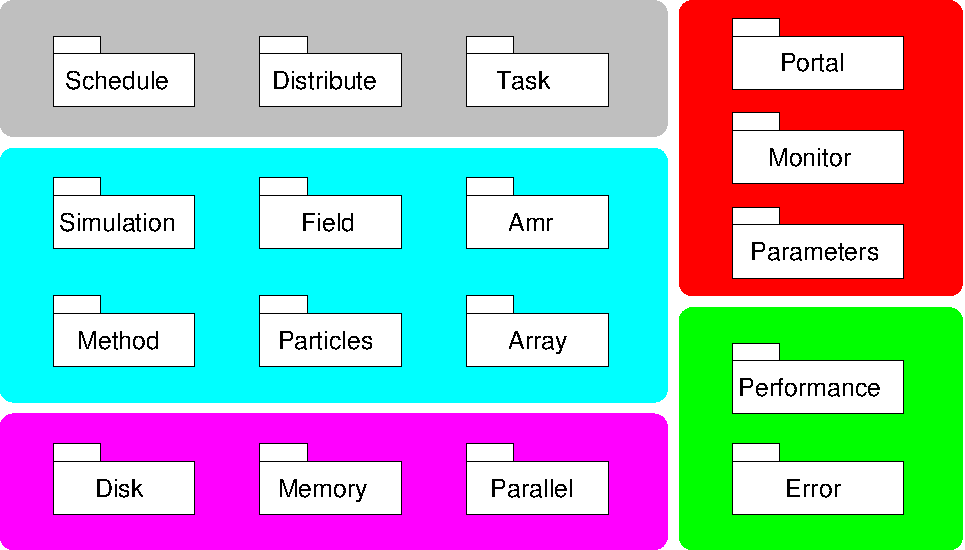
\includegraphics[width=5.0in]{components2.pdf}
\end{minipage}}

The high-level components include \code{Task} for encapsulating
parallel tasks, \code{Distribute} for distributing and load-balancing
tasks across available resources, and \code{Schedule} for scheduling
the tasks for execution.

The middle-level components include \code{Simulation} for defining the
simulation, and \code{Method} for user functions for
performing the numerical computations, inline analysis, and
visualization processing required to run the simulation.  Distributed
AMR is implemented in the \code{Amr} package, with related components
\code{Field} and \code{Particles} for representing data fields and
particle groups defined on the AMR hierarchy.  \code{Array} is a
component for defining and manipulating distributed Fortran-like
arrays.

The low-level components include API's for interacting with hardware,
including \code{Disk} for disk I/O, \code{Memory} for dynamic memory
management, and \code{Parallel} for parallel synchronization and data
transfer.  Including these lower level components is helpful for
several reasions: it encapsulates lower-level library calls, e.g.~HDF5
for \code{Disk}, which can include extra functions for collecting
performance data; it allows for incorporating error checking code,
e.g.~ tracking memory usage and performing bounds checking in
\code{Memory}; and parallel technologies such as MPI, UPC, and OpenMP
can be encapsulated in \code{Parallel}.

Components implementing cross-cutting concerns include
\code{Parameters} for reading, storing, and accessing parameters,
\code{Monitor} for logging performance and status information, and
\code{Portal} for dynamically interacting with external utilities or
systems.  \code{Performance} is used for collecting and accessing
performance-related data, and \code{Error} is used for signalling
hardware or software faults.

Component sizes will vary: \code{Amr} is expected to be large since
representing and manipulating distributed AMR hierarchies is
inherently complex, whereas \code{Memory} is likely to be relatively
small.  Larger components will be further decomposed into smaller
sub-components, e.g.~\code{Amr} may contain \code{Tree}, \code{Patch},
\code{Level}, and \code{Box} subcomponents, to help organize and
control software complexity.  Larger components may be implemented
using several interacting class hierarchies, whereas smaller
components may be implemented as a single class.

Below in sections \S\ref{ss:design-amr} through
\S\ref{ss:design-resilience} we describe preliminary design issues
related to requirements listed in sections \S\ref{ss:require-amr}
through \S\ref{ss:require-resilience}, respectively.

\newpage
%-----------------------------------------------------------------------
\subsection{Adaptive mesh refinement} \label{ss:design-amr}
%-----------------------------------------------------------------------

How adaptive mesh refinement is designed is crucial for it to meet the
scaling requirements outlined in \ref{ss:require-amr}.  It must
maintain high parallel efficiency throughout the range of single-level
``unigrid'' problems, through ``wide'' problems requiring millions of
patches, and ``deep'' problems requiring several dozens of levels.
All must be efficiently mapped to HPC architectures with millions of
cores with fixed physical memory capacity per node.

The most important AMR data structure design decision is what variant
of AMR to use.  The two leading variants are ``block-structured AMR
(SAMR)'', or patch-based AMR, as used by \samrai\ and \chombo; and
``continuous AMR (CAMR)'', or octree-based AMR, as used by \paramesh.
There are numerous advantages and disadvantages to each, and
significant effort has gone into deciding which approach to pursue.
We have decided on a modified octree-based AMR approach, with two
modifications that improve AMR efficiency for both ``wide'' and
``deep'' problems.  We review these two modifications below.

We feel that octree-based approaches are arguably more
scalable~\cite{BuGh08}, in part because they avoid the parallel patch
placement algorithms required by SAMR, which are a significant
hinderance to scalability~\cite{GuWi06}.  Also, high quality SAMR
frameworks such as \chombo\ and \samrai\ are already available and
being actively developed.  Lastly, the octree in octree-based AMR can
be leveraged for particle neighbor searches; octrees have particularly
efficient representations and operations (e.g.~an octree node can be
stored using three pointers~\cite{@@@octree}); and absolute patch
extents are computed not stored, which can be used to address
precision and range issues of global indices that arise for extremely
large or deep AMR hierarchies.

@@@@@@@@@@@@@@@

Standard octree-based approaches involve an octree or forest of
octrees.  Nodes of the octree typically correspond to small fixed-size
locally Cartesian grid blocks, such as the $4^3$ grid blocks used in
the FLASH astrophysics application built on the \paramesh\ framework.


\begin{verbatim}
   AMR operations
     initial grid generation
     refinement criteria: tag refine or coarsen
     refine or coarsen
     octree-specific: balance
     parallel distribution and redistribution
     access to associated fields, particles
     access to neighbors, parent, children
        for interpolate fields
     block-structured-specific: parallel clustering algorithm
\end{verbatim}

\begin{verbatim}
Octree AMR starting point
Remaining issues and solutions
  1. fixed-sized grid patches for large unigrid areas
     ``Coalescing'' optimization
  2. ``shallow'' refinemet for deep
     ``Targeted refinement with backfill''
  3. global indices
      option for relative coordinates for patches   
  4. global time steps
      Patch-local adaptive time steps
  5. replicated data
      Hybrid replicated / distributed  data structure

Related issues
   Load balancing: \ref{ss:design-balance}
   Task definition and scheduling: \ref{ss:design-schedule}
Next: mesh and particles
\end{verbatim}

@@@@@@@@@@

\textbf{Patch coalescing}. One proposed enhancement to the typical
octree-based AMR approach is to allow variable mesh sizes per AMR
hierarchy patch.  This can be introduced using the simple invertable
AMR-invariant operation illustrated in Figure~\ref{f:coalesce}.  While
keeping the underlying mesh resolution constant, the operation
transforms multiple AMR patches with a single patch, but with a larger
mesh.  We call this \textit{patch coalescing}.  The inverse operation
is permitted as well if the patch requires subsequent refinement or
coarsening.

\FIGURE{Coalescing}{f:coalesce}{
\begin{minipage}{3.75in}
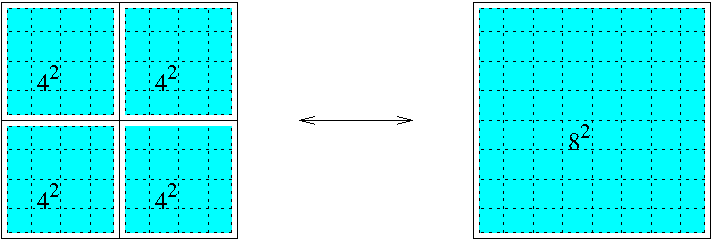
\includegraphics[width=3.75in]{coalesce.pdf}
\end{minipage}}


This operation decouples the AMR topology from the local resolution
requirements, which permits a more efficient AMR data structure for
the same resolution requirement.  Patch coalescing will be
particularly efficient for AMR problems that involve large regions
in which the resolution is uniform.  We note that this modification
is not relevant to block-structured AMR, since patch sizes are already
variable.

As a proof-of-concept, below in Figure~\ref{f:cosmo} is an image of a
2D cosmology density field projection, together with two balanced 2D
quadtrees adapted to the image's gray scale.  One of the quadtrees
used fixed-resolution patches, whereas the other used patch
coalescing.  Even though the example problem is not particularly
well-suited for this technique, it nevertheless leads to a quadtree
with $2 1/2$ times fewer nodes.

\FIGURE{ Coalesced patches proof-of-concept using a 2D cosmology
  density field projection.  \textbf{Left}: 2D cosmology density field
  projection.  \textbf{Middle}: Balanced quadtree with 81701 patches.
  \textbf{Right}: Balanced quadtree with 32529 coalesced patches. \\
} {f:cosmo}{
\begin{minipage}{7.0in}
\begin{minipage}{2.2in}
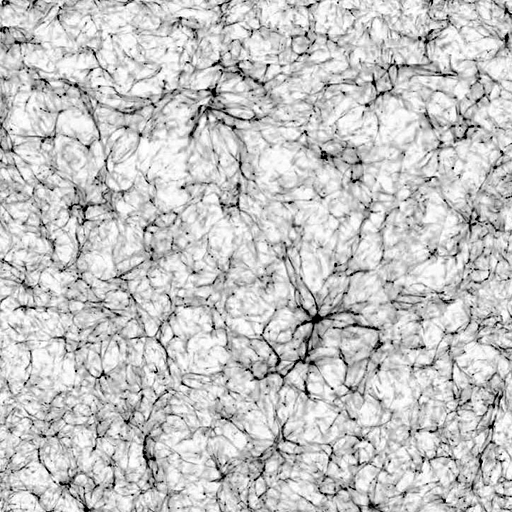
\includegraphics[width=2.2in]{cosmo2-invert.png}
\end{minipage} \ 
\begin{minipage}{2.2in}
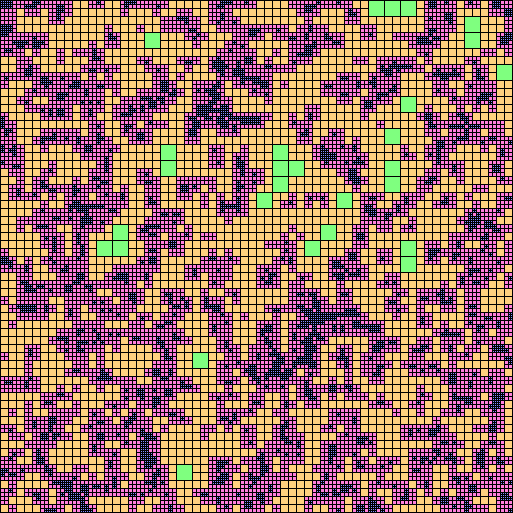
\includegraphics[width=2.2in]{cosmo2-4-1-inv.png}
\end{minipage} \ 
\begin{minipage}{2.2in}
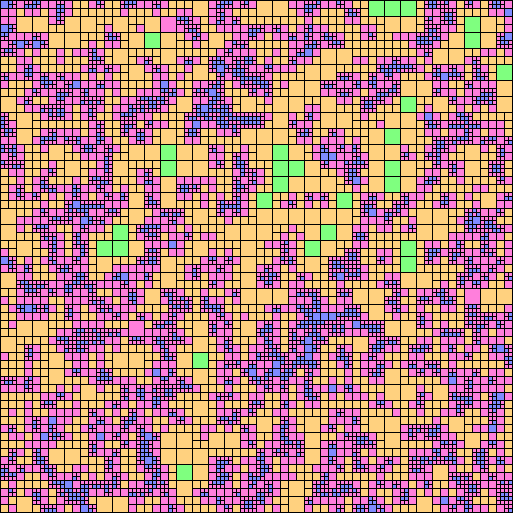
\includegraphics[width=2.2in]{cosmo2-4-2-inv.png}
\end{minipage}
\end{minipage}
}

While allowing flexible patch block sizes can greatly reduce the size
of the octree-based AMR data structure, the variable block size can
complicate other issues, specifically load balancing and parallel task
definition.  Load balancing is complicated since work load per grid
patch is no longer ``constant'' within a level (though we argue later
that it is not necessarily constant to begin with), and task
definition is complicated by the wide variation in task size.  We
address this issue by decoupling parallel tasks from AMR patch blocks,
essentially by allowing parallelism within a patch block.  With this
approach, which we describe in more detail in
\S\ref{ss:design-schedule}, we can maintain a constant subblock task
size despite permitting arbitrarily large AMR patch blocks.


%------------------------------------------------------------------------

\textbf{Targeted refinement}.  Another proposed enhancement to the
octree-based AMR approach is, instead of using a $2^3$-tree (octree)
and refining by $r=2$, we use a $4^3$-tree and refine by $r=4$, or an
$8^3$-tree and refine by $r=8$.  We call this $r^3$-tree approach
\textit{targeted refinement}.

The motivation and main advantage of targeted refinement is for
particularly deep AMR runs, where the region of interest is tiny
relative to the global domain size, such as simulations of galaxy or
star formation.  As a proof-of-concept example, in Figure~\ref{f:dots}
two balanced $r^2$-trees are shown refined on a small set of points in 2D, one
with $r=2$ and one with $r=4$.

\FIGURE{
Targeted refinement proof-of-concept using multiple point sources in 2D.
\textbf{Left}: 2D point sources.  
\textbf{Middle}: Balanced octree with 2137 patches.
\textbf{Right}: Balanced octree with 158 explicit patches.
}
{f:dots}{
\begin{minipage}{7.0in}
\begin{minipage}{2.2in}
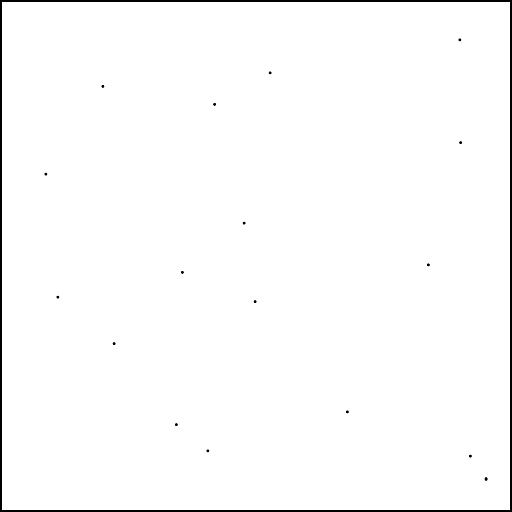
\includegraphics[width=2.2in]{dots-invert.png}
\end{minipage} \ 
\begin{minipage}{2.2in}
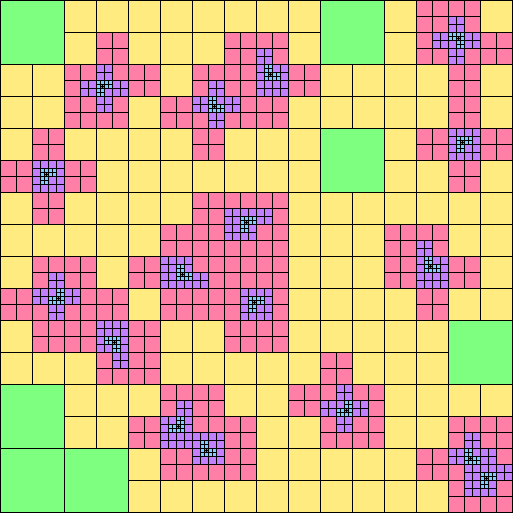
\includegraphics[width=2.2in]{dots-4-1-inv.png}
\end{minipage} \ 
\begin{minipage}{2.2in}
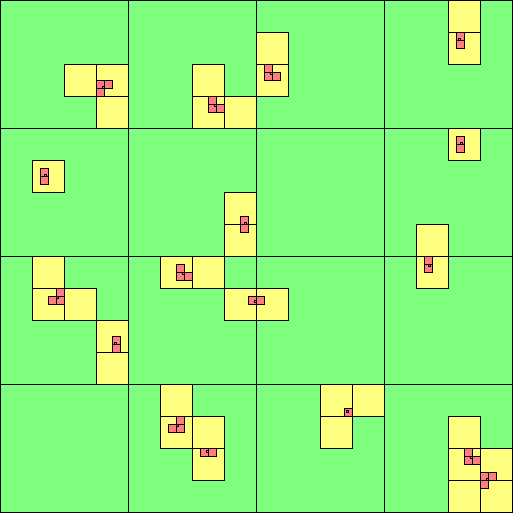
\includegraphics[width=2.2in]{dots-16-5-inv.png}
\end{minipage}
\end{minipage}}

The advantage is clear: the number of nodes in the AMR hierarchy is
reduced by a factor of about $13.5$.  There are apparent disadvantages
as well.

One disadvantage is that balancing an $r^3$-tree still allows jumps in
refinement greater than two.  We can regain this mesh constraint by
introducing implicit \textit{backfill} patches, as indicated in
Figure~\ref{f:backfill}.

\FIGURE{Targeted refinement with backfill}{f:backfill}{
\begin{minipage}{6.15in}
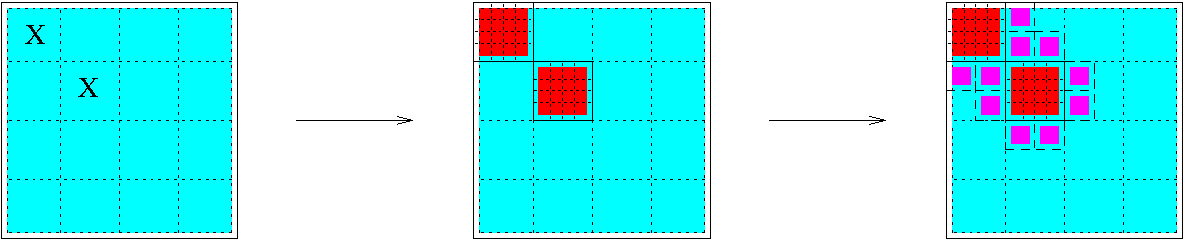
\includegraphics[width=6.15in]{kd-backfill.pdf}
\end{minipage}}

Another disadvantage is that we need to represent the $r^3$-trees.
This can be done by simply using the $2^3$-tree data structure
implementation and ignoring intermediate levels.  This still reduces
the overall data structure size, since the balancing step is only
performed on the ``active'' levels.  This can also improve parallel
scaling: the $2^3$-tree balancing operation potentially affects all
levels of the hierarchy,.whereas for $r>2$ the $r^3$-tree balancing
and backfill operations are more localized.

%------------------------------------------------------------------------

\textbf{Delete coarse levels}.  For particularly
deep AMR runs, the simulated time of interest can be much less
than the time steps at the coarser levels.  If it is known that
data at a coarse level is no longer required, that level can
simply be removed from the simulation, freeing up resources for
finer levels.  In principle, this could allow arbitarily deep AMR runs,
provided other data structure limits and numerical scaling is
handled appropriately.


\begin{verbatim}
2. AMR algorithm enhancements: targeted refinement by 4 or 8
   improves ``deep'' AMR
   refinement by 2 too ``shallow''
   back filling possible to regain effect of balanced tree
   sparse storage format of child patches to reduce storage 
   balancing octrees can have global effect
     balancing refinementy by 4 or 8 probabalistically (provably?) local
     no explicit AMR patches required for backfill--can live on child nodes 
     EXAMPLE: point refinement
   targeted refinement by 4 or 8
     especially effective for deep AMR, e.g. star formation with
       30+ levels
     still supports effective resolution jumps of 2 using backfill
     still representable with octree data structure 
        skip intermediate levels
        add additional backfill patches
   Note refining single point introduces global refinement back to coarse level
      effects entire domain even for infinitely localized point
\end{verbatim}



%------------------------------------------------------------------------
\textbf{Implicit global indices.}

\begin{verbatim}
3. option for relative coordinates for patches   
   relative to neighbors
   hydro computations generally only require local cell size and time step
      global indices an issue for deep AMR due to limited precision: limit scalability
         ``eliminate integer precision dependence on data structure size''       
      no stored global indices
         compute absolute coordinates only when necessary using octree structure
            compute to required precision
            initialization
            inline analysis
            global position dependent physics
               e.g. internal boundaries or fixed sources or sinks
               not necessarily supported by the initial framework
      global: computed with octree
      distributed: only position relative to neighbors
  only need mesh width and time step size for advancing
  localization an option--not needed for smaller problems
  use similar localization approach for particles, described in \ref{ss:design-particles}
\end{verbatim}

%------------------------------------------------------------------------

\textbf{Patch-local adaptive time steps}. There are two common
variants in time step determination: uniform time steps over the
entire domain, and adaptive time steps at each refinement level.
These variants have their relative advantages and disadvantages:
adaptive time steps are more computationally efficient, especially for
``deep'' AMR runs, whereas using uniform time steps is more scalable
since all patches can advance a time step simultaneously.

One disadvantage of both is that determining the time step, either for
the entire domain or within individual levels, requires a global
reduction operation.  However, global operations are particularly costly for
massively parallel machines.  

We believe this global operation can be avoided by relaxing the
constraint of a fixed time step within a level.  The time step is
determined to a large part by the spacial resolution of the mesh,
which is constant within a level; however, in highly dynamic regions
such as rapid gravitational collapse, the local physics may lead to
requiring a smaller time step.  Instead of allowing these isolated
regions to determine the time step for the entire level, we will
optionally permit individual patches to make multiple time steps
relative to other patches in the same level.  For some problems, this
may help prevent rapidly evolving feature in one localized region of
the domain from determining the time step everywhere else.


%------------------------------------------------------------------------

\textbf{Distributed data structure.} There are two main approaches
used for representing the AMR hierarchy structure on a distributed
memory machine: storing part of the hierarchy on each process, and
storing the entire hierarchy on all nodes or processes.

Each clearly has its advantages and disadvantages.  Duplicating the
entire hierarchy on all processes can be more efficient, since
operations involving the hierarchy as a whole may require no
communication.  However, the approach ultimately does not scale, since
available memory per process is always limited, so as the problem size
growes, eventually the AMR data structure storage will consume all
available memory.

Our solution, which has been used by others
(e.g.~\cite{@@@hybrid-storage}), will be to support both, by
duplicating coarser levels of the octree, and distributing the finer
levels.

\begin{verbatim}
5. Hybrid replicated / distributed  data structure
   For each local grid patch, only immediate neighbors and
     ancestors stored
     Proxies for remotely stored patches
       remote thread identifier + pointer
   Replicated as well as distributed
     Hybrid: top k levels replicated
   Replicated option: reduce tree-AMR node size
      only storing parent, child, data pointer \cite{@@@
      SAMR patches indexed by single-precision offsets into parent
      patches, 32 bytes / tree-AMR and 48 bytes / patch-AMR]
   distributed AMR hierarchy
      local patches: store parent, neighbors, children (sparse)
      not as memory efficient as globally stored nodes 
         (3 pointers, 24 bytes average)
         cite (petascale AMR?)
      proxies for remotely stored patches
  For each patch, only store patch, location information for
    neighboring patches (``ghost patches''), and ancestors for octree
\end{verbatim}

@@@@@@@


%-----------------------------------------------------------------------
\subsection{Mesh data} \label{ss:design-fields}
%-----------------------------------------------------------------------

\begin{verbatim}
[review requirements]
User-controlled optional floor/ceiling limits on individual
  Fields (ala ``tiny\_number'' in Enzo), with user-specified Error
  behavior (warning, error, ignore, reset to given floor/ceiling,
  etc.)
support coordinate rescaling at deep levels
Units
\end{verbatim}

%-----------------------------------------------------------------------
\subsection{Particle data} \label{ss:design-particles}
%-----------------------------------------------------------------------

\begin{verbatim}
[review requirements]
Store particle positions in single precision as -1 <=  x,y,z <= 1
  relative to their containing patch. [To reduce storage, improve
  performance, and address precision issues with deep AMR.]
Use a binary tree data-structure to recursively partition the
  bounding boxes of particles.
  absolute particle positions / grid locations may be needed
     for some output, e.g. global particle analysis
  in that case low precision
\end{verbatim}

\begin{verbatim}
patch-local coordinates for particles
   control accumulation of roundoff
   minimize / eliminate effects of limited precision and range
   absolute coordinates computed when necessary
      analysis
      visualization
\end{verbatim}

\begin{verbatim}
particles
   groups of related particles stored together
   particles associated with grid patch
   flexibility in particle ownership
     may belong to immediate neighbor to reduce communication
particle positions stored using local coordinate system with
  origin at patch corner
\end{verbatim}


%-----------------------------------------------------------------------
\subsection{User functions} \label{ss:design-user}
%-----------------------------------------------------------------------

\begin{verbatim}
Integrate ``inits'' functionality into the main code
Declarative rather than imperative
   define actions
   define dependencies
   system determines order to do things
   support override?
user functions supplied
   method ``checkin'' or initialization functions
      identify by name (for performance and monitoring)
      defines fields required
         variable ghost zone depths
      defines particle groups required
         levels of ghost zones
      type: hydro, elliptic
      any parameters required
      any other data required for checkpointing
      ... 
      any temporary method-local fields / particles required
      any static  method-local fields / particles required
      data layout of fields expected (can be interleaved, etc.)
   define method sequence within a level (hydro then gravity)
   define method sequence between levels (flux correction)
   field / particle initialization
   particle advance
   particle computation
   particle - grid interaction
   block advance (multiple)
   inter-level flux correction
   refine / coarsen
   time step determination
   constraint enforcement (div B)
   error checking / invariant checking for fault tolerance / software resiliency
      detects memory / cpu errors and mark core as faulty and bypass
      API provided for signalling errors
 
   field and data ghost zones available
      can be different for different fields
      can be different for different methods
   hydro support:
       advance single block a single time step
       full data including ghost fields and ghost particles available 
          see Schedule
   elliptic support:
       solver on single level or entire hierarchy
       parallelism?
       how to implement?
   global and level operations / solves
Support optional uniform time steps across all levels. [To
  improve parallel efficiency.]
Support optional variable time step sizes within each level. [To
  reduce synchronization costs when computing global CFL condition.]
\end{verbatim}


\begin{verbatim}
Support ensembles within a single run, including inline-analysis
\end{verbatim}

%-----------------------------------------------------------------------
\subsection{Run-time parameters} \label{ss:design-parameters}
%-----------------------------------------------------------------------

The parameter component is currently implemented and functional.

[wiki]

[devel]


%-----------------------------------------------------------------------
\subsection{Parallelism} \label{ss:design-parallel}
%-----------------------------------------------------------------------

@ 1 charm mode

@ 2 reasons [requirements]

@ 3 other technologies \& reasons [hierarchical]

We plan to support a variety of parallelization technologies and
paradigms from the start.  These technologies will including message
passing via the MPI library~\cite{wwwmpi}, partitioned global address
space (PGAS) programming via the UPC~\cite{@@@UPC} language, shared
memory parallel programming via OpenMP~\cite{@@@OpenMP} compiler
directives, processor virtualization via the \charm\
framework~\cite{@@@Charm}.  Select hybrid approaches will also be
supported, including MPI with OpenMP, and MPI with UPC.  While
heterogeneous platforms, such as those containing general purpose
graphics processing units (GPGPU's), will not be directly supported,
but the framework's design will facilitate their use by the
user-written physics kernels.

There are several reasons why we plan to include multiple
parallelization technologies.  First, because the performance and
scalability of the technologies vary between machines and
implementations~\cite{MaTa09}, and we want to always use the fastest
and most scalable approach.  Second, one technology may perform better
in the distributed memory regime, whereas another may perform better
within a shared memory node, which motivates flexible hybrid parallel
approaches.  Third, by including multiple existing parallelization
paradigms from the start, the resulting software design will likely be
more amenable to incorporating new parallelization technologies that
may be developed in the future.  And fourth, the framework could be
used as a tool for parallel technology designers and implementers to
compare and improve their approach with other existing approaches on
new and existing hardware platforms.

Our approach to including multiple parallelization technologies will
be to abstract out the concept of a parallel task: an entity that runs
on a single computational component, and which may have dependencies
with other tasks.  Defining, balancing, and executing tasks will be
performed by the high-level components \code{Task}, \code{Distribute},
and \code{Schedule}.  Low-level parallel operations required for task
migration, synchronization, and data transfer will be implemented in
the \code{Parallel} component.  We expect the component will include
two parallelization API's, one for distributed memory and one for
shared memory.  The distributed memory API would encapsulate MPI and
UPC, whereas the shared memory API would encapsulate OpenMP and UPC.

This approach is most similar to the process virtualization model used
by \charm, the functionality of which subsumes that of all three of
our high level \code{Task} (``chare''), \code{Distribute}, and
\code{Schedule} components~\footnote{We note that \charm\ also
  supports checkpointing for fault-tolerance, and performance
  monitoring and visualization, which we may encapsulate in our
  \code{Error} and \code{Performance} components.}  This similarity is
no coincidence, since the \charm\ model helped influence our
high-level parallelization design.  Because of this close match in
design, we will therefore begin parallel development using the
high-level \charm\ framework.  Later development will include
supporting MPI, UPC, and OpenMP for hierarchical and hybrid
parallelism, and will reuse code kernels required for \charm, e.g.~for
``packing'' and ``unpacking'' task-related data for migration.

We are also considering encapsulating data communication between tasks
as a task itself, so that scheduling of communication can be
integrated with scheduling of computation.  The motivation is that it
could improve performance, while reducing memory cost in communication
buffers and code complexity.

\begin{verbatim}
Reduce implicit dependencies by dynamically allocating parallel
  tasks, ala \charm. (e.g. currently Enzo loops through patches within
  a level, but a given patch can proceed as soon as it has all its
  boundary data)
\end{verbatim}

\begin{verbatim}
Only use inter-core, inter-cpu, inter-node, etc.
  level-communicators to bound communicator size and manage
     communication nonuniformity.
  motivates MPI,UPC,OpenMP
\end{verbatim}

\begin{verbatim}
Support multiple (hybrid) and flexible parallelization
  strategies, including MPI-1 (2-sided send/recv), MPI-2 (1-sided
  get/put), OMP, and optionally UPC and GPU.
hierarchical synchronization and collective operations
\end{verbatim}

\begin{verbatim}
memory storage formats and data movement
   Amr data stored for memory and operations; restructure for comp and comm
   Compute in reformatted ``computational registers'' (Block class in Array)
      basic idea used in \paramesh
         ``working block'' 
         ``work'' datastructures
      can alias with Amr if ghost zones stored to avoid copy
      particle types collected / distributed
   Communicate using reformatted ``flux registers''
      idea used in \chombo: \code{LevelFluxRegister}
      can alias with fields if ghost zones stored to avoid copy
      can alias with particles 
        pointer per particle?  
        pointer / length per particle sub array
\end{verbatim}
 
\begin{verbatim}
Scheduling optimized for computing / communication
     compute block size optimized for cache
        copied to array compute registers
        blocking/padding for cache / memory hierarchy
        groups of blocks for GPU / fp accelerators
     more flexible:
        arbitrary reordering of array axes
        arbitrary subset of axes
        arbitrary ghost zone depth
          more adaptable to existing legacy ``unigrid'' routines
          different reorderings possible for different methods (hydro, chemistry, etc.)
          flexibilty allows improved data-layout for single-thread performance
             cache blocking, padding
   scheduler reuse for computation / communication scheduling
\end{verbatim}

%-----------------------------------------------------------------------
\subsection{Load balancing} \label{ss:design-balance}
%-----------------------------------------------------------------------

Dynamic load balancing is well known to be a crucial operation for
extreme scalability in general, and for extreme adaptive mesh
refinement in particular.  Computational load must be evenly
distributed to maintain high overall parallel computational
efficiency; dynamically allocated memory must be well-distributed
across compute nodes to avoid running out of physical memory; and data
locality must be maintained within compute nodes to maintain high
communication performance over the interconnect.

A highly scalable approach of rebalancing octree-based SAMR
hierarchies is to linearize the data structure using a Morton, Gray
code, or Hilbert type space-filling curve, then partition the tree
nodes among processes by dividing the linearized structure into $N_P$
evenly sized pieces.  This approach has been shown to scale to over
$60K$ cores~\cite{@@@ART}.  It works well if workload and memory usage
are proportional to each other within tree nodes, and when workload
between tree nodes is roughly equal; however, neither of these
conditions is met when adaptive time steps are used.  Also, this
approach still requires $O(N_P)$ storage, and a global all-gather
operation (e.g.~\code{MPI\_Allgather}) is required on all processes.

Our approach will be to 

\begin{verbatim}
 load balancing
    hierarchical
       improved scalability
       improved flexibility
       improved efficiency
    distribution approaches
       replicated
       distributed
       hybrid
         optimize computational performance versus memory usage
     
    load balance locally in given level
    different metrics at different levels
      memory at node level
      workload below
    different frequency at different levels
      lower frequency balancing at higher levels
         more costly
         solution changes less frequently
      higher frequency balancing at lower levels
         less costly
         solution changes more frequently
    task adjacency maintained
    use collected performance data
    explore overcompensation technique
       ala SOR
       two regimes
          local collapsing / explosion
          shock advancement
       identify regimes and adapt
    linearized Morton, Gray code, Hilbert curve insufficient
       assumes equal work per patch
       particles are associated with nodes, changing weight
       adaptive time steps drastically weights more highly  refined patches
       performance of physics algorithms on a patch is not necessarily uniform
          localized chemistry subcycling, front tracking, etc.
       arrays on patches may be different sized (assuming coalesced patches)
       linearization constricts dimensionality
          constrains data movement along a single dimension
          physics imbalances 4 dimensional
      Morton ordering not always feasible
         different particle counts
         adaptive time steps on finer levels
         physics method variations
            shock capturing--Riemann solver iterations
            variable subcycling of iterative stiff methods
\end{verbatim}


\begin{verbatim}
task migration
   migrate tasks dynamically
   Charm++ model: pack, relocate, unpack data
   maintain locality by moving task to owner of a neighbor
   maintain parent-child locality when possible
      relax for deep hierarchies
   migrate using hierarchical parallelism
\end{verbatim}
\begin{verbatim}
Load-balance using ``over-compensation'', since heavily-loaded
  processes tend to continue to become more heavily loaded (cosmology
  / star-formation application-dependent).
\end{verbatim}

(e.g.~load balancing
across $\approx 2^20$ cores can be replaced by four hierarchical
load balancing steps across $\approx 2^5$)


for each node, and if the global \code{MPI\_AllGather} of long
integers on $N_C$ cores is acceptable \footnote{\cite{BuGh08}
  indicates $N_C$ cores, though we believe with a hybrid programming
  approach their global reduction could be reduced to an even more
  scalable $N_P$ MPI processes}.  However, we anticipate that this
approach will not be sufficient for a general-purpose extreme AMR
framework for several reasons.
%
One, adaptive time steps are required for efficient ``deep'' AMR
problems, but that scales the work load for a given node by a
non-constant factor of roughly $2^k$ for level $k$.
%
Two, particle distributions among nodes may not be uniform, affecting both memory and computational loads.
%
Three, array patches may be differently sized, if we use our ``coalesced patches'' enhancement to reduce the AMR tree node count.  
%
Four, performance of physics methods on a patch is not necessarily
uniform, due to, e.g., localized subcycling of stiff methods, front
tracking methods, etc.  The first three issues, and possibly the
fourth, could be addressed by dynamically weighting nodes before
partitioning them among processes, but that would require additional
global communication to perform the reduction.
%

Lastly, we suspect that linearizing the workload artificially
restricts the flexibility of data movement allowed (along one
dimension instead of three), creating more communication traffic
during task migration.  than in not be optimal in terms of the amount
of data that needs to be redistributed during each rebalancing step,
since it restricts workload along a single dimension, whereas the
actual workload is typically distributed along three or four
dimensions (three spacial and one time).

Since we suspect that a space-filling curve approach is only effective
for a strict subset of AMR problems we wish to support, we will
explore two ideas for dynamic load balancing, including ``hierarchical
load balancing'', and a new approach we call ``deliberate
overcompensation''.

\note{load-balancing: hierarchical} 
%
By \textit{hierarchical load balancing} we mean rebalancing tasks
between higher levels (nodes or supernodes) independently from
rebalancing between lower levels (socket or cores).  The idea of
hierarchical task scheduling and load balancing has been known for at
least 15 years (\cite{AhGh94}, but is not commonly used for AMR
frameworks.

This will have several advantages over more traditional
non-hierarchical load balancing.  First, rebalancing at different
levels could be based on different metrics, e.g. memory usage for
rebalancing between nodes, and computational load for rebalancing
between sockets.  This will be particularly useful for AMR problems,
because memory is the crucial metric we want to keep balanced at the
node level, yet we want to balance computational time at lower
hardware platform levels to keep computational elements busy.  Second,
rebalancing frequencies at different levels can be decoupled,
rebalancing less frequently at the upper node levels where rebalancing
is more costly, and where load tends to take longer to become
unbalanced.

\note{load-balancing: deliberate overcompensation}
%
By \textit{deliberate overcompensation} we mean rebalancing by
relocating \textit{more} than enough tasks from high-load to low-load
processes.  The motivation is for physics phenomena, such as
gravitational collapse or explosions, that require a continuous and
regular redistribution of computational resources.  The idea is
conceptually analagous to the successive over-relaxation (SOR) variant
of the Gauss-Seidel method.  This approach could potentially reduce
the frequency of rebalancing the load by half with the same tolerance
on imbalance.

%
\note{load-balancing: data locality}
Data locality is crucial for parallel performance, so tasks associated
with neighboring patches and parent-child patches are kept on the same
process when possible, or failing that, on ``close'' processes (same
socket or node) if possible.  This will be maintained by weighting
migration of tasks to closer processes (through hierarchical load
balancing), and migrating a task to another process only if a
neighbor, parent, or child of the task is associated with that
process.  This will enforce the spacial data associated with tasks
assigned to a process to be simply connected.  We also wish to keep
the surface area-to-volume ratio low.  The space-filling curve
approach is a specialization of maintaining simply connectednes, and
we expect the additional generalization can be used to improve data
locality, surface-to-volume ratio, and reduce task migration traffic.

``diffusion-based scheme''

% \begin{verbatim}
% OOP
%   addresses 
%     agility, readability, flexibility, modifyability, extensibility, complexity
%   improves component reuse, controls software
%   complexity, eases software maintenance
%   still not always ideal
%      cross-cutting components
%      can use aspect-oriented ideas
%   design patterns
% \end{verbatim}
% 



%-----------------------------------------------------------------------
\subsection{Task scheduling} \label{ss:design-schedule}
%-----------------------------------------------------------------------

Given that tasks are acceptably load-balanced across process, the
tasks must be schedule for execution.  The @@@

\begin{verbatim}
dynamic scheduling
\end{verbatim}

\begin{verbatim}
task definition Task
   task = grid patch block (fields and particles) + sequence of methods
      increased scheduling freedom over loop over levels
      improves slack for latency hiding
   elliptic tasks?
\end{verbatim}

\begin{verbatim}
   tradeoff between number of concurrent messages and storage
      dynamic allocation of flux buffers
\end{verbatim}

\begin{verbatim}
   communication tasks scheduled with computation
      prefetch comm
      pipeline comm and comp
\end{verbatim}

\begin{verbatim}
   prioritized queue: fine levels higher priority
      determine rate of progress: bottleneck
\end{verbatim}

\begin{verbatim}
hierarchical / multiscale task scheduling
   multiblock (GPU)
   single block (process)
   plane / line (thread)
\end{verbatim}

\begin{verbatim}
   Store only actual data
     use flux registers for communication
     allocate patch ghost zones only for computation
     Support temporary ``allocate as-needed'' ghost zones
        in addition to ``permanent'' ones
     optimized for storage: Amr
        option to not store guard / ghost cells
        AMR patches may be larger than computationally optimal
   Could store appropriate subset of neighbor data as well for
     fault-tolerance
\end{verbatim}

We will use dynamic scheduling of tasks assigned to a processes, since
it @@@  Dynamic scheduling is more suitable than static scheduling for
heterogeneous sized tasks, non-regular communication dependencies @@@

\note{task scheduling details}

After tasks are distributed among processing elements, the next
decision is how to schedule tasks among processing elements.  Two main
approaches are static and dynamic.  Static scheduling is preferred
when workload is evenly mapped to processing components, and when
there are relatively few tasks per process.  We will use dynamic
scheduling, since workload (communication as well as computation) per
task varies between tasks.

\note{Charm++ summary} Our approach will be well-mapped to \charm,
which is a fault-tolerant message-driven parallel programming
framework.  \charm\ also provides dynamic load balancing through task
migration, and provides fault tolerance through its built-in disk (or
memory + disk) checkpoint / restart mechanism.

\note{implementation in Charm++}
Implementation of AMR for a hyperbolic problem, a parallel task, or
\charm\  ``chare'', would correspond to advancing a numerical method or
sequence of methods one time step on a single grid patch block.  The
exchange of guard cell data would correspond to \charm\  messages.
This implementation would allow a block to advance one time step as
soon as all of its guard cell data is available.

\note{non-Charm++ implementation}

We also plan to develop our own scheduler, for several reasons.  One,
to schedule communication in addition to computation, to help hide
latency through prefetching.  Second, to take advantage of
hierarchical hardware components (node, socket, core...)  Third, to
remove any hard dependencies on any single parallel technology.



%-----------------------------------------------------------------------
\subsection{Interfaces} \label{ss:design-interfaces}
%-----------------------------------------------------------------------

%-----------------------------------------------------------------------
\subsection{I/O} \label{ss:design-io}
%-----------------------------------------------------------------------


\begin{verbatim}
I/O different output formats for different uses
   checkpointing
   analysis
   visualization
   general ``data dump''
   cheaper to rerun and regenerate data to process than dump and reread later
      inline analysis capability to reduce overall output required
   checkpoints
       node / processor independent: software resiliency
       checkpoints restartable on different configurations / platforms
   ``accessor code'' included with all output data
\end{verbatim}
\begin{verbatim}
I/O
   parallel HDF5
   compression
   CRC error-checking and retry
   subset of nodes do I/O
   detection of faulty disk and mark as unusable
   different formats for different uses
\end{verbatim}

\begin{verbatim}
Enforce strict control over data storage formats (e.g. files)
  (see W0009)
Require that all stored data be accessed through standard
  interface functions that are independent of specific file formats
  (i.e., stored datasets are conceptually treated as objects)
\end{verbatim}

%-----------------------------------------------------------------------
\subsection{Performance} \label{ss:design-performance}
%-----------------------------------------------------------------------

\begin{verbatim}
integrated performance monitoring
   summaries at different hardware levels
   less frequent at lower levels--more data
   more frequent at upper levels
   performance data available to other components
      load balancing based on actual memory usage / cpu time
      feedback for adaptivity
      help identify performance and scaling issues early
      poor-performance resilient
\end{verbatim}

\code{Portal} Component

\begin{verbatim}
portal: support interfacing with other codes
   post-processing solvers
   data analysis pipeline
   visualization pipeline
      use existing library, e.g. Visit
      Method can include visualization or inline analysis
\end{verbatim}

\code{Monitor} Component

\begin{verbatim}
monitor: support for interfacing with user while running
   ``dashboard'' for real-time monitoring state of simulation
\end{verbatim}


% \begin{verbatim}
% hybrid parallel
%    MPI + OMP
%    MPI + UPC
%    UPC + OMP (?)
%    Charm++ + OMP (?)
%    flexible subset of cores, sockets, nodes, supernodes
%    Task scheduling Charm++ model, but implemented in MPI, UPC, OMP
%    processor-task affinity
% \end{verbatim}

% \begin{verbatim}
% Charm++ 
%   data placement
%   load balancing
%   task scheduling
%   checkpointing for fault tolerance
%   performance monitoring and visualization
% \end{verbatim}

\begin{verbatim}
platform hierarchical architecture-aware data structures
  e.g. MPI communicator for cores in a socket, sockets in a
    node, nodes in a supernode, supernodes in a machine
  facilitates hierarchical dynamic load balancing
    improves dynamic mapping of data structures to hardware components
    E.g. load balance more frequently at core / socket level to
      keep functional units busy
    load balance node / supernode levels less frequently to keep
      memory usage uniform
    less frequent because:
      problem changes less at larger scales
      rebalancing is more expensive: larger data sizes, slower
        interconnects
    user-defined parameters and metrics for load balancing at
      different levels
      dynamically collected performance data can be fed back
        into hierarchical load balancing algorithm
  note linearization of octree datastructure is insufficient:
    assumes equal work per patch
    particles are associated with nodes, changing weight
    adaptive time steps drastically weights more highly
      refined patches
    performance of physics algorithms on a patch is not
      necessarily uniform, e.g. localized chemistry subcycling, front
      tracking, etc.
    arrays on patches may be different sized
    linearization of patches 
        reduces flexibility
        constrains data movement along a single dimension
\end{verbatim}

\begin{verbatim}
Multiple parallelization strategies
  MPI: + widespread, optimized implementations, familiar
  MPI: - data replication, difficult to use
  UPC + easier to use, combines shared memory view with efficient data affinity
  UPC - no concept of MPI communicator, still under development--not as mature
  OMP + can be used progressively
  OMP - not scalable outside of socket / node;  inefficiencies due to false cache sharing
  GPU + very fast / power efficient when usable
  GPU - no usable standard, difficult to program, difficult to map problem to hardware
  Charm++ + higher-level, dynamic scheduling, dynamic load-balancing, fault tolerant through checkpointing to other node memory
  Charm++ - requires learning separate language, separate runtime system, no data prefetching(?)
    currently not fully realizable for GPU since depends on
      computational code
    hierarchical parallelism: MPI + OMP, MPI + UPC, MPI + GPU,
      etc.
    advantages of hybrid
      reduced data replication from MPI distributed memory
      dynamic parallel threads--use more when helpful, fewer when not
      UPC
    disadvantages of hybrid
      performance hit from data sharing in MPI + OMP
      MPI and UPC communication cannot (currently) proceed concurrently
    code for two modes: distributed memory and shared memory
    parallel tasks: grid patches, arrays, grid patch groups,
      particle groups
    flexible data structure parameters (grid patch size, patch
      decomposition, patch grouping) to dynamically optimize task size
\end{verbatim}

\begin{verbatim}
hierarchical parallelism
   encourage communication within hardware components
      sockets within node
      cores within socket
      hyperthreads within core
\end{verbatim}

\begin{verbatim}
parallel technology encapsulation / processor virtualization
  distributed / shared memory
    MPI (two-sided and one-sided) (distributed memory)
    OpenMP (shared memory) 
    UPC (either distributed memory or shared memory)
    Charm++
  multiple strategies enhance software resiliency
    i.e. buggy MPI implementation--dynamically switch to UPC
\end{verbatim}

%-----------------------------------------------------------------------
\subsection{Resilience} \label{ss:design-resilience}
%-----------------------------------------------------------------------

\pargraph{fault tolerance} Fault tolerance and software
resilience are crucial factors at extreme scales, since it has been
observed that frequency of failures is proportional to the number of
sockets~\cite{@@@}

\begin{verbatim}
 FT-MPI 
  ``fault-tolerante MPI''
  http://icl.cs.utk.edu/ftmpi/overview/index.html 
MPICH-V 
  ``MPI Implementation for Volatile resources''
  http://mpich-v.lri.fr/index.php 
\end{verbatim}


\begin{verbatim}
software resilience
   take advantage of only Methods change data
   methods signal which fields / particles changed
\end{verbatim}
\begin{verbatim}
fault-tolerance / software resilience strategies
   need to deal with continuous stream of failures
   MTTF < MTTC
   checkpoint to disk
      issue: failures will become more frequent than time to checkpoint
      agressively reduce checkpoint data size and write time
         dedicated I/O nodes
         compress
         check data
         methods identify which data modified
            may help lower disk output--only checkpoint modified data
   checkpoint to memory
     Charm++ does this(?)
   detect hardware errors and mark as defective
       memory
       disk
       core
       socket
       node
       interconnect (pairs of nodes)
       software libraries (MPI versus UPC, etc.)
   flash memory
   log faults to disk for subsequent analysis
   performance resilience
      dynamically adapt to reduce cache thrashing / ineffeciency
          array blocking or padding in computational array registers
      adapt AMR patch size, refinement factor (2,4,8)
   fault-tolerant MPI
      FT-MPI
   leverage new approaches when available
      active research area
      keep up to date in latest practices
      design software to use new approaches
\end{verbatim}


%=======================================================================
\section{Implementation} \label{s:implementation}
%=======================================================================


\begin{verbatim}
   Programming environment
     Trac
        wiki for developing design
        browser for viewing source code
        roadmap for organizing milestones
        tickets for defining tasks and tracking defects
   Editor
      xemacs
      Eclipse?
   Source code     
      currently subversion
      likely move to mercurial
   Documentation
      Doxygen
      Latex for 
\end{verbatim}

\begin{verbatim}
   Development approach
     requirements, design, implement, test
        developed on Trac wiki
        formalized in Latex documents
   Iterative
      begin with core functionality
      iterate on added functionaly
      ensure correct at each iteration
      quick iterations avoid spending too much time in any one step
   Heavy emphasis on designing before coding
     easier to change requirements than design, design than code
     explore new ideas before implementing them
     prototyping useful as approximate ``predictor step'' of final design
\end{verbatim}
\begin{verbatim}
iterative development
   requirements, design, implementation, tests, user documentation updated in sequence
\end{verbatim}



\begin{verbatim}
application driven
   helpful for ensuring completeness
      missing functionality in design will become apparent
   helpful for testing
   \enzoii\ 
   cosmology / astrophysics
   requires wide range of AMR capabilities
     broad for galaxy structure formation
     deep for star formation
     turbulence
   requires wide range of physics capabilities
     hyperbolic: hydrodynamics
     elliptic: self-gravity, FLD radiation
     local physics: chemistry, heating/cooling
   decouple physics modules from AMR framework
   make both \enzoii\  and underlying AMR framework publicly available
\end{verbatim}

\begin{verbatim}
currently primarily in early requirements capturing and high-level 
        design phase
   available flexibility to modify current design
   design as described is current snapshot
   little code and time wasted
emphasis on thorough designing before coding
   prototype ideas before final implementation
   more time upfront known to lead to faster overall development times
\end{verbatim}

\begin{verbatim}
   Components
      correspond to a source code directory
      may have subcomponents
      User code provided as overriden Method classes
      Only Fortran or C required of user
      Minimal C++ required for application developer
   Interdependencies  
      controlled at component and class level
      correspond to \code{#include "component.h"}
   Classes
      access functions used instead of direct attribute access
   Rapid prototyping
      proof-of-concept
      explore software designs
\end{verbatim}

\begin{verbatim}
  Languages
    Framework: C++
       components, subcomponents, classes
       composition preferred to inheritance
    Parallelization
       isolated CHARM++, UPC, C99 + OpenMP directives
       MPI library
    User code
       C, C++, Fortran 
       CUDA / OpenCL / etc (user code only)
\end{verbatim}

\begin{verbatim}
  Libraries
     I/O: HDF5
     random: SPRNG, user-defined
\end{verbatim}

\begin{verbatim}
  Configuration
    Minimal compile-time configuration for library availability
    Precision is run-time option
    Field-by-field precision override
\end{verbatim}

\begin{verbatim}
   Building
      Currently GNU make
      Possibly add GNU Autotools
      Explore Ant or SCons
\end{verbatim}


\begin{verbatim}
   Documentation
      source code: Doxygen
\end{verbatim}



%=======================================================================
\section{Quality Control} \label{s:testing}
%=======================================================================

No single method of improving software quality finds all defects, so
we will employ a set of techniques that have been proven in practice
to be successful~\cite{Mc04}.  These include unit testing, integration
testing, regression testing, beta testing, code reviews, design reviews, and
refactoring.

Defects can be costly, but they are much more costly when found later
in the development cycle.  Defects can occur in any phase of the
development cycle, but those in earlier phases (requirements and
design) tend to be much more costly than those in later phases
(implementation and testing).  Although we We therefore concentrate on quality
control more heavily our effort on earlier phases.

It is well known that improving the quality of software reduces the overall
development costs. 
 phasesWe therefore
approach to quality control is to concentrate on all phases of the
development cycle.  software development approach is to 
concentrate on 

Software in general is difficult to develop in part because it
involves a litany of desirable characteristics determining its overall
quality: software should be maintainable, flexible, portable,
usable, reusable, readable, testable, understandable, efficient, correct,
reliable, adaptable, accurate, robust, etc.  These characteristics
depend on decisions made during the development process, so design
and implementation decisions must be made deliberately and thoughtfully.


\begin{verbatim}
   Improving quality reduces development costs
      defects costly, especially later in development cycle
      time spent in finding and preventing defects well worth it
         more time spent testing and reviewing can paradoxically
         reduce overall development time
   Testing + design and code reviews (collaborative construction)
      Testing complement reviews [CITE code complete]
      may try pair programming
   Refactoring to reduce code complexity
      continually refactor
      rigorous testing
   Testing approach
      unit test all code
      regression testing
          use lcatest parallel testing framework
          correctness, performance, scaling, resilience
          correctness
             \enzoii\  implementation
             compare agains Enzo I results
             existing test problems
          performance
             built-in performance monitoring
             single-thread
             weak and strong parallel scaling 
             communication performance
             I/O performance
          scaling
             extreme broad problems (grid / particle counts)
                cosmology
             extreme depth problems
                star formation
          software resilience
             memory, compute, network, disk, algorithms
             memory failures
                fill
                load balancing for memory
             compute failures
                tag component (cabinet, node, socket, core) as unusable
             network failures
                checksums
                reroute P1->P2 as P1->Pj->P2
             disk failures
                checksums
             algorithm failure
                support adaptive algorithms
                locally override spacial mesh width / time steps
   Software reviews
      line-by-line checking
         by another person, or after time elapsed
   Refactoring
development
   implement progessively to fill user beta testing pipeline
\end{verbatim}

\begin{verbatim}
testing
   lcatest: automated parallel application testing
   multiple test levels
      unit tests
      component tests
      application tests
      in-house / community beta-testing
         (progressive as functionality comes online)
   test for multiple things:
      functionality
      correctness
      performance
      scaling
   tests also help supplement user documentation
   use integrated performance monitoring
      PAPI for hardware counters
      PMPI for MPI communication
      new[] / delete[] overload for dynamic memory usage
         particularly important for AMR
      user-defined independent attributes
         cycle
         level
         process
      user-defined dependent metrics
         process-local patch counts
         process-local cell / zone counts
         process-local particle counts
      less frequent output at finer levels (more data)
   helps identify functional, performance, scaling bugs early
   extreme scaling designed into framework from the start
\end{verbatim}

%=======================================================================
\section{Development Plan} \label{s:plan} 
%=======================================================================

\begin{verbatim}
  Charm++ generalized unigrid
     evaluate effectiveness
  AMR hyperbolic
  particle methods
  AMR elliptic
\end{verbatim}

%=======================================================================
\section{Milestones and Deliverables} \label{s:milestones}
%=======================================================================

\begin{verbatim}
   Cello software framework
   research papers
   Complete \enzoii\  application
   large-scale demonstration using \enzoii
   workshop/training
\end{verbatim}

%=======================================================================
\bibliography{papers}
\bibliographystyle{unsrt}
%=======================================================================

\end{document}

%==================================================================

